\section{Theoretische Grundlage}
\label{sec:Theorie}

Ziel dieses Versuches ist es mit Hilfe verschiedener Brückenschaltungen unbekannte Wiederstände, Kapazitäten und Induktivitäten auszumessen. Dies wird zum Beispiel mittels einer Abgleichbedingung realisiert.
Jede Brückenschaltung wird prinzipiell von einer Speisepannung $U_\text{s}$ und vier Wiederständen betrieben. Dies kann auch durch Scheinwiederstände realisiert werden, was impliziert das die Brückenschaltung je nach Aufbau mit Wechselstrom betrieben werden muss.
\begin{figure}
	\centering
	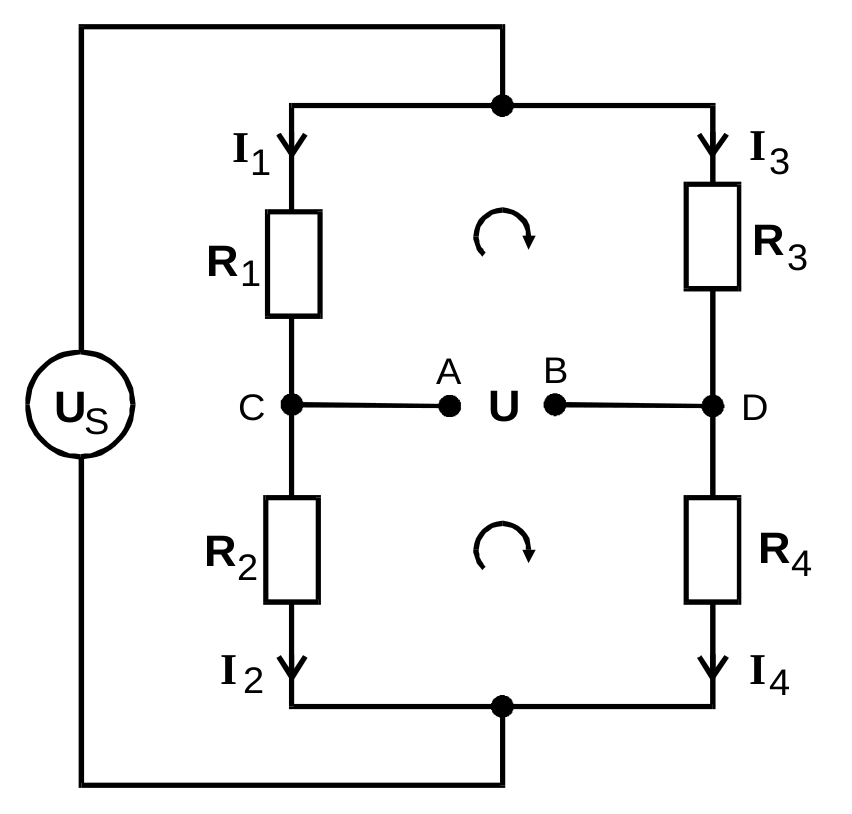
\includegraphics[height=5cm]{picture/1.png}
	\caption{wesentlicher Aufbau einer Brückenschaltung}
	\label{fig:wheatstone}
\end{figure}
Die Brückenschaltung liegt dem Kirchhoffschen Regeln zu Grunde. Die erste der beiden Regeln besagt, das die Summe der eingehenden und ausgehende Ströme an eineme Knoten gleich Null ist.
\begin{equation}
  Knotenregel : \sum_{\text{k=1}}^\text{n} I_\text{k} = 0
  \label{eqn:K1}
\end{equation}
Die zweite Regel besagt, dass bei einer Geschlossenen Masche sich alle Teilspannungen, bei einem Umlauf zu Null addieren.
\begin{equation}
  Maschenregel : \sum_{\text{k=1}}^\text{n} U_\text{k} = 0
  \label{eqn:K2}
\end{equation}
Unter Berücksichtigung der Kirchhoffschen Gesetzen ergibt sich für die einfachste Brückschaltung eine Brückenspannung $U_\text{Br}$ von 
\begin{equation}
  U_\text{Br} = \frac{R_2 R_3 - R_1 R_4}{(R_3 + R_4)(R_1 + R_2)} 
  \label{eqn:Ubr} 
\end{equation}
Es wird das Wiederstandverhältnis so gewählt das die Brückenspannung minimal wird. Daraus ergibt sich die Abgleichsbedingung 
\begin{equation}
  R_2 R_3 = R_1 R_4 \ .
  \label{eqn:R}
\end{equation}
Dabei können die Wiederstände auch komplex sein. Dabei kommt es jedoch zu Phasenverschiebungen.

\subsection{Wheatstone Brücke}
Die Wheatsonte Brücke besteht ausschließlich aus Wiederständen. Sie ist dafür gedacht einen Unbekannten Wiederstand $R_\text{x}$ mittels der oben genannten Abgleichmethode zu bestimmen. Der Schematische Aufbau einer Wheatsone Brücke ist in Abbildung \ref{fig:widerstand} zu sehen. 
\begin{figure}
      \centering
      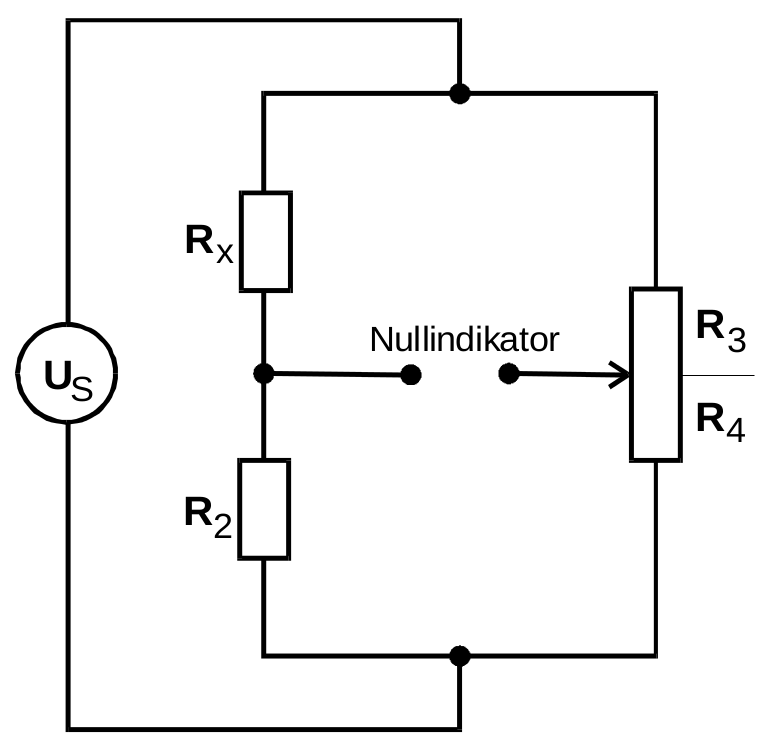
\includegraphics[height=5cm]{picture/2.png}
      \caption{wesentlicher Aufbau einer Brückenschaltung}
      \label{fig:widerstand}
\end{figure}
Durch umstellen der Gleichung \ref{eqn:R} erhält man für die den gesuchten Wiederstand $R_\text{x}$ die Formel, 
\begin{equation}
  R_x = R_2 \frac{R_3}{R_4} \ .
  \label{eqn:R_x}
\end{equation}
Das Verhältniss $R_3$ zu $R_4$ lässt sich besonders gut mit Hilfe eines Potentiometer einstellen.
\subsection{Kapazitätsmessbrücke}
Mit dieser Messbrücke soll die Kapazität des Kondensators bestimmt werden. Dies geschieht über die Impedanz des Kondensators, daher muss der Aufbau mit Wechselstrom betrieben werden. Da es sich im Versuch um keinen idealen Kondensator handelt wird im Schaltbild ein fiktiver Widerstand $R_\text{x}$ vor den Kondensator geschaltet.
\begin{figure}
  \centering
  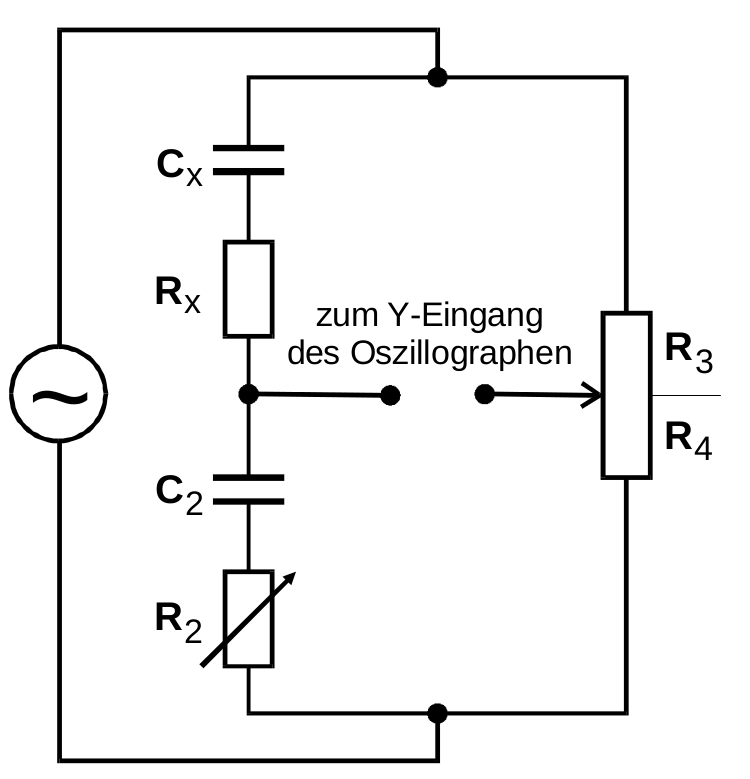
\includegraphics[height=5cm]{picture/3.png}
  \caption{Messung der Kapazität eines realen Kondensators}
  \label{fig:C}
\end{figure}
Mittels der Abgleichbedingung gibt sich analog zu Formel \ref{eqn:R_x} ein Widerstand von 
\begin{equation*}
    R_x = R_2 \frac{R_3}{R_4} \ ,
\end{equation*}
und für den Kondensator unter berücksichtigung der Scheinwiderstände
\begin{equation}
  C_x = C_2 \frac{R_4}{R_3} \ .
  \label{C_x}
\end{equation}

\subsection{Induktivitätsmessbrücke}
Mittels der Messbrücke aus der Abbildung \ref{fig:L} soll die Induktivität einer Spule bestimmt werden. Dies geschieht Analogie zur Kapazitätsmessbrücke über die Impedanz der Spule,daher muss der Aufbau mit Wechselstrom betrieben werden.

\begin{figure}
  \centering
  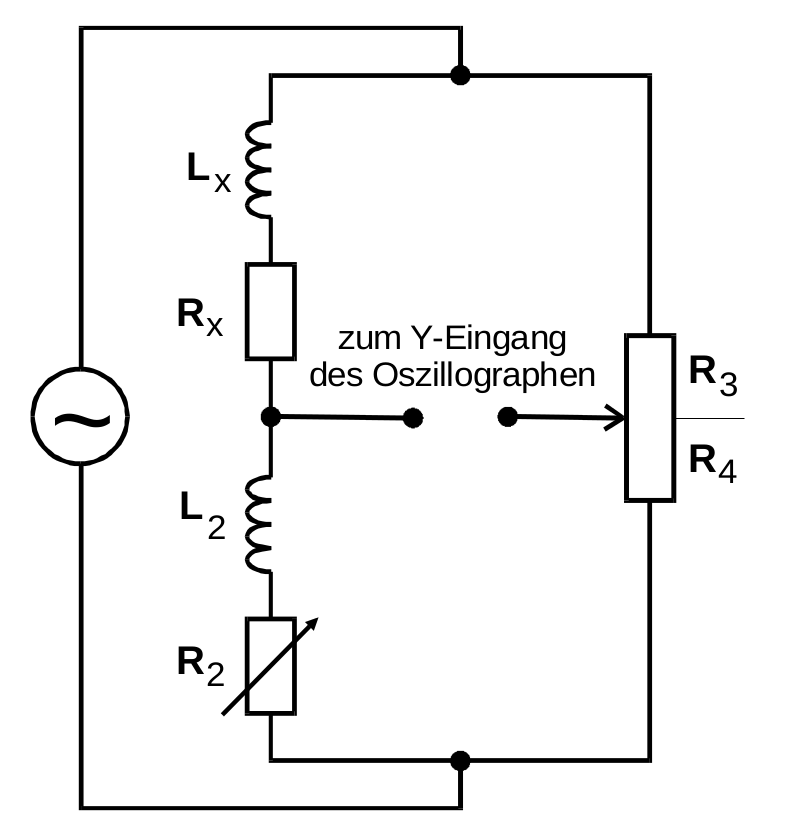
\includegraphics[height=5cm]{picture/4.png}
  \caption{Messung der Induktivität einer realen Spule}
  \label{fig:L}
\end{figure}
Mittels der Abgleichbedingung gibt sich analog zu Formel \ref{eqn:R_x} ein Widerstand von
\begin{equation*}
     R_x = R_2 \frac{R_3}{R_4} \ ,
\end{equation*}
und für den Kondensator unter berücksichtigung der Scheinwiderstände
\begin{equation}
   L_x = L_2 \frac{R_4}{R_3} \ .
   \label{C_x}
\end{equation}
\subsection{Maxwell-Brücke}
Es soll die Induktivität einer Spule mit Hilfe der Maxwell-Brücke bestimmt werden. Dafür wird anstelle einer Spule, wie im vorherigen Kapitel beschrieben, ein Kondensator verwendet und wie in Abbildung \ref{fig:Max-Br} aufgebaut. Es muss darauf geachtet werden, dass einerseits, die Frequenz hoch genug ist, damit sich der Einschwingvorgang hinreichend schnell einstellt und andererseits die Frequenz niedrig genug ist, damit die Streukapazitäten niedrig genug sind um einen Abgleich zu ermöglichen.
\begin{figure}
  \centering
  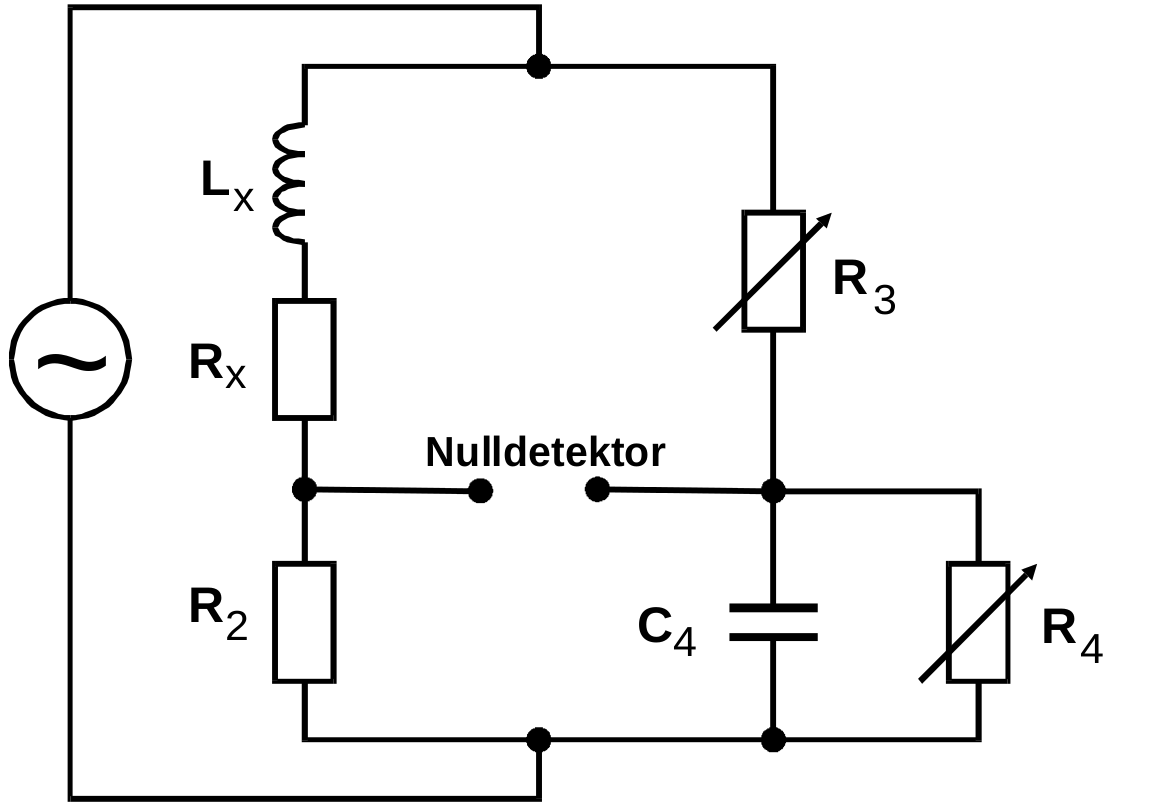
\includegraphics[height=5cm]{picture/5.png}
  \caption{Messung der Induktivität durch eine Maxwell-Brücke}
  \label{fig:Max-Br}
\end{figure}
Mit Hilfe der Maschenregel ergeben sich die Gleichungen zu Bestimmung der Induktion 
\begin{equation}
  L_x = R_2 R_3 C_4
  \label{eqn:L_x}
\end{equation}
sowie für den fiktiven Wiederstand
\begin{equation}
  R_x = \frac{R_2 R_3}{R_4}
  \label{eqn:R_M}
\end{equation}

\subsection{TT-Brücke}
Mittels einer TT-Brücke soll die Funktion des elektrischen Filters genauer bestimmt werden. Dafür wird die Schaltung Abbildung \ref{fig:TT} entsprechend aufgebaut.
\begin{figure}
  \centering
  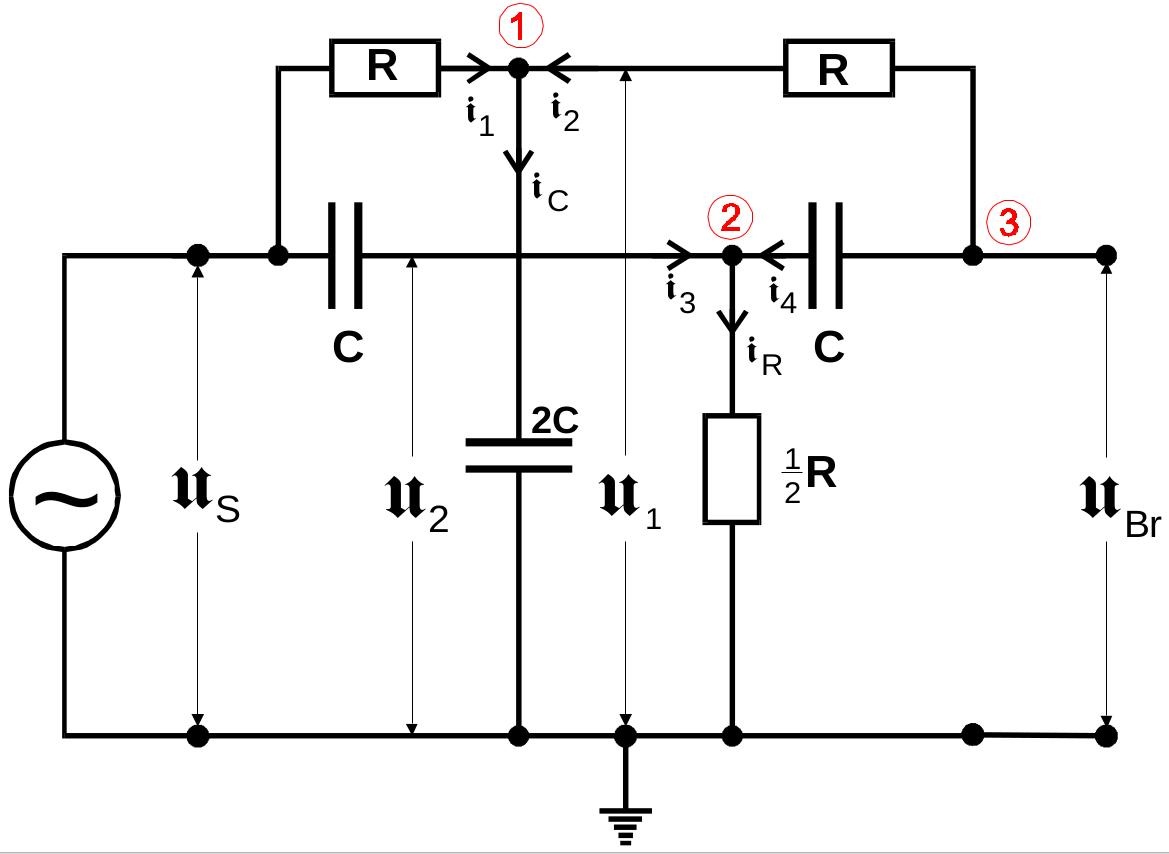
\includegraphics[height=5cm]{picture/7.png}
  \caption{Messung der Induktivität durch eine TT-Brücke}
  \label{fig:TT}
\end{figure}
Das Spannungverhältniss $U_\text{Br}$ zu $U_\text{S}$ zu berechnen werden die Ströme an den Knoten 1, 2 und 3 betrachtet. Für den ersten Knoten ergibt sich nach der Kirchhoffschen Knotenregel
\begin{equation}
  \frac{U_1 - U_\text{S}}{R} + \frac{U_1 - U_\text{Br}}{R} = 2 j \omega C U_1 \ .
  \label{eqn:M1}
\end{equation}
Mit Hilfe der Ströme an dem zweiten 
\begin{equation}
  \left( U_\text{S} - U_2 \right) j \omega C + \left( U_\text{Br} - U_2 \right)j \omega C = \frac{2}{R} U_2
  \label{eqn:M2}
\end{equation}
und dritten Knoten
\begin{equation}
  \left( U_2 - U_\text{Br} \right)j \omega C + \frac{U_q - U_\text{Br}}{R} = 0
  \label{eqn:M3}
\end{equation}
lässt sich durch Auflösen der Gleichungen \ref{eqn:M1}, \ref{eqn:M2} nach $U_1$ und $U_2$ und deren Ergebnisse in \ref{eqn:M3} eingesetzt, die Brückenspannung ermitteln.
\begin{equation}
  U_\text{Br} = U_\text{S} \frac{1 - \omega^2 R^2 C^2}{1 - \omega^2 R^2 C^2 + 4 j \omega R C}
  \label{eqn:Ubr}
\end{equation}
Als Spannungsverhältniss erhält man durch umstellen der Gleichung \ref{eqn:Ubr} und der Einführung von 
\begin{equation*}
  \Omega = \omega R C
\end{equation*}
die Form 
\begin{equation}
  \frac{U_\text{Br}}{U_\text{S}} = \frac{1 - \Omega^2}{1 - \Omega^2 + 4 j \Omega} \ .
  \label{BrS}
\end{equation}

\subsection{Fehlerrechnung}
Sämtliche Fehlerrechnungen werden mit Hilfe von Python 3.4.3 durchgeführt.
\subsubsection{Mittelwert}
Der Mittelwert einer Messreihe $x_\text{1}, ... ,x_\text{n}$ lässt sich durch die Formel
\begin{equation}
	\overline{x} = \frac{1}{N} \sum_{\text{k}=1}^\text{N} x_k
	\label{eqn:ave}
\end{equation}
berechnen. Die Standardabweichung des Mittelwertes beträgt
\begin{equation}
	\Delta \overline{x} = \sqrt{ \frac{1}{N(N-1)} \sum_{\text{k}=1}^\text{N} (x_\text{k} - \overline{x})^2}
	\label{eqn:std}
\end{equation}

\subsubsection{Gauß'sche Fehlerfortpflanzung}
Wenn $x_\text{1}, ..., x_\text{n}$ fehlerbehaftete Messgrößen im weiteren Verlauf benutzt werden, wird der neue Fehler $\Delta f$ mit Hilfe der Gaußschen Fehlerfortpflanzung angegeben.
\begin{equation}
	\Delta f = \sqrt{\sum_{\text{k}=1}^\text{N} \left( \frac{ \partial f}{\partial x_\text{k}} \right) ^2 \cdot (\Delta x_\text{k})^2}
	\label{eqn:var}
\end{equation}

\subsubsection{Lineare Regression}
Die Steigung und y-Achsenabschnitt einer Ausgleichsgeraden werden gegebenfalls mittels Linearen Regression berechnet.
\begin{equation}
	y = m \cdot x + b
	\label{eqn:reg}
\end{equation}
\begin{equation}
	m = \frac{ \overline{xy} - \overline{x} \overline{y} } {\overline{x^2} - \overline{x}^2}
	\label{eqn:reg_m}
\end{equation}
\begin{equation}
	b = \frac{ \overline{x^2}\overline{y} - \overline{x} \, \overline{xy}} { \overline{x^2} - \overline{x}^2}
	\label{eqn:reg_b}
\end{equation}
